\section{ガウス過程$^\ddagger$}

$N$次元ガウシアン分布を
\begin{align}
    \Ng(\xv;\muv, \Sigma) \equiv \dfrac{1}{\sqrt{(2 \pi)^{N} |\Sigma|}} e^{- (\xv - \muv)^\top \Sigma^{-1}(\xv - \muv) /2  }
\end{align}
と表記する。また誤解がない場合、変数$\xv$を略して、
\begin{align}
    \Ng(\muv, \Sigma) \equiv \dfrac{1}{\sqrt{(2 \pi)^{N} |\Sigma|}} e^{- (\xv - \muv)^\top \Sigma^{-1}(\xv - \muv) /2  }
\end{align}
のように表記する場合もある。

\subsection*{相関ノイズとしてのガウス過程}
ガウス過程は、多変数正規分布
\begin{align}
\dv \sim \Ng(\zerov,\Sigma)
\end{align}
に従う確率変数$\xv$の確率過程のことである。いま$d_i$は時系列だとして、この多変数正規分布の共分散行列の各成分が、
\begin{align}
\Sigma_{ij} = K_{ij}(a, \tau) = a k(|t_i-t_j|; \tau)
\end{align}
のように、$t_i$と$t_j$の差の絶対値の関数として与えられれば、相関長$\tau$のガウス過程が得られる。
カーネル関数$k(t,\tau)$としてはいろいろなタイプがありうるが、例えばRBFカーネル
\begin{align}
 k_\mathrm{RBF}(t;\tau) = \exp{\left(- \frac{t^2}{2 \tau^2} \right)},
\end{align}
とMat\'{e}rn 3/2カーネル
\begin{align}
\label{eq:MaternA}
 k_\mathrm{M3/2}(t;\tau) = \left( 1 + \frac{\sqrt{3} t}{\tau} \right) e^{- \sqrt{3} t/\tau}. 
\end{align}
などがある。

このガウス過程にしたがったデータ点をサンプリングしてみると図\ref{fig:gp1}のようになる。ただしデータにさらに平均ゼロ、標準偏差$\sigma$のガウスノイズを足している。このノイズを便宜的に観測ノイズと呼んでおこう。
\begin{figure}[htb]
\begin{center}
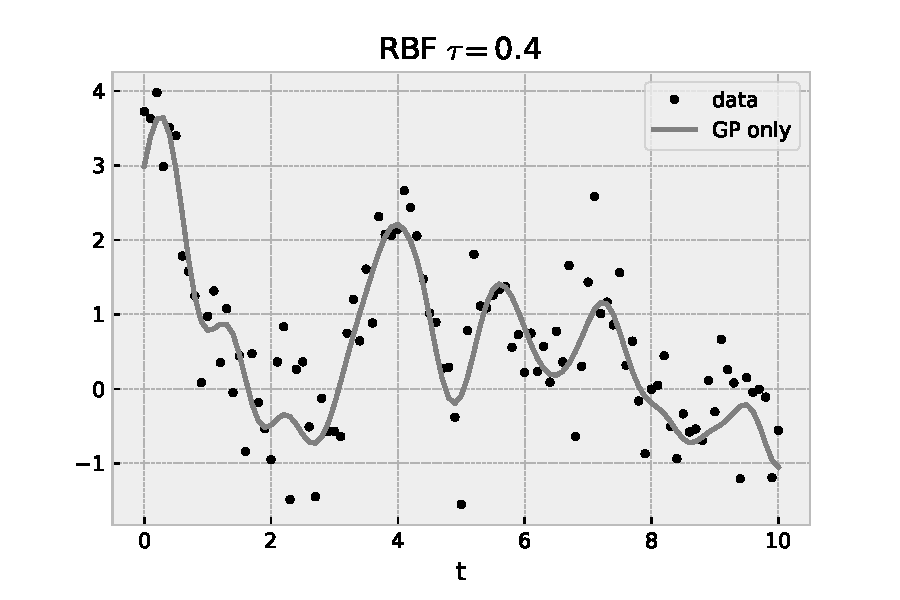
\includegraphics[width=\linewidth]{fig/gp/gp1.pdf}
\caption{ガウス過程からサンプルされたデータ。実線は$\sigma$の観測ノイズなし。\label{fig:gp1}}
\end{center}
\end{figure}



さてこのデータを元に$\tau$、$a$、$\sigma$をMCMCサンプリングしてみよう。平均ゼロ、標準偏差$\sigma$のガウスノイズの観測ノイズを足したということは確率モデルとしては、
\begin{eqnarray}
\label{eq:gpmodel0}
\dv &\sim& \Ng(\zerov,\Sigma^\prime ) \\
\Sigma^\prime &=& K(a, \tau) + \sigma^2 I
\end{eqnarray}
となる。この$\Sigma^\prime$はRBFカーネルを仮定し、さらに独立誤差を表す対角項を加える。つまり
\begin{align}
 \Sigma_{ij} (a, \tau, sigma) = a k_\mathrm{RBF} (|t_i - t_j|; \tau) + \sigma^2 I
\end{align}
となり、共分散はパラメタ$(a, \tau, \sigma)$を持つ。Exponential分布$E(x)$を用いて事前分布を構成すると、たとえば事前分布は
\begin{align}
    p(a) &= E(1) \\
    p(\tau) &= E(1) \\
    p(\sigma) &= E(1) 
\end{align}
となり、尤度は
\begin{align}
    p(\dv|a, \tau, \sigma) = \Ng(\zerov,  \Sigma (a, \tau, \sigma) )
\end{align}
のようにかける。つまりこれでMCMCを回すことができる。


HMCでサンプルした事後分布を可視化したものが図\ref{fig:gp2}である。
\begin{figure}[htb]
\begin{center}
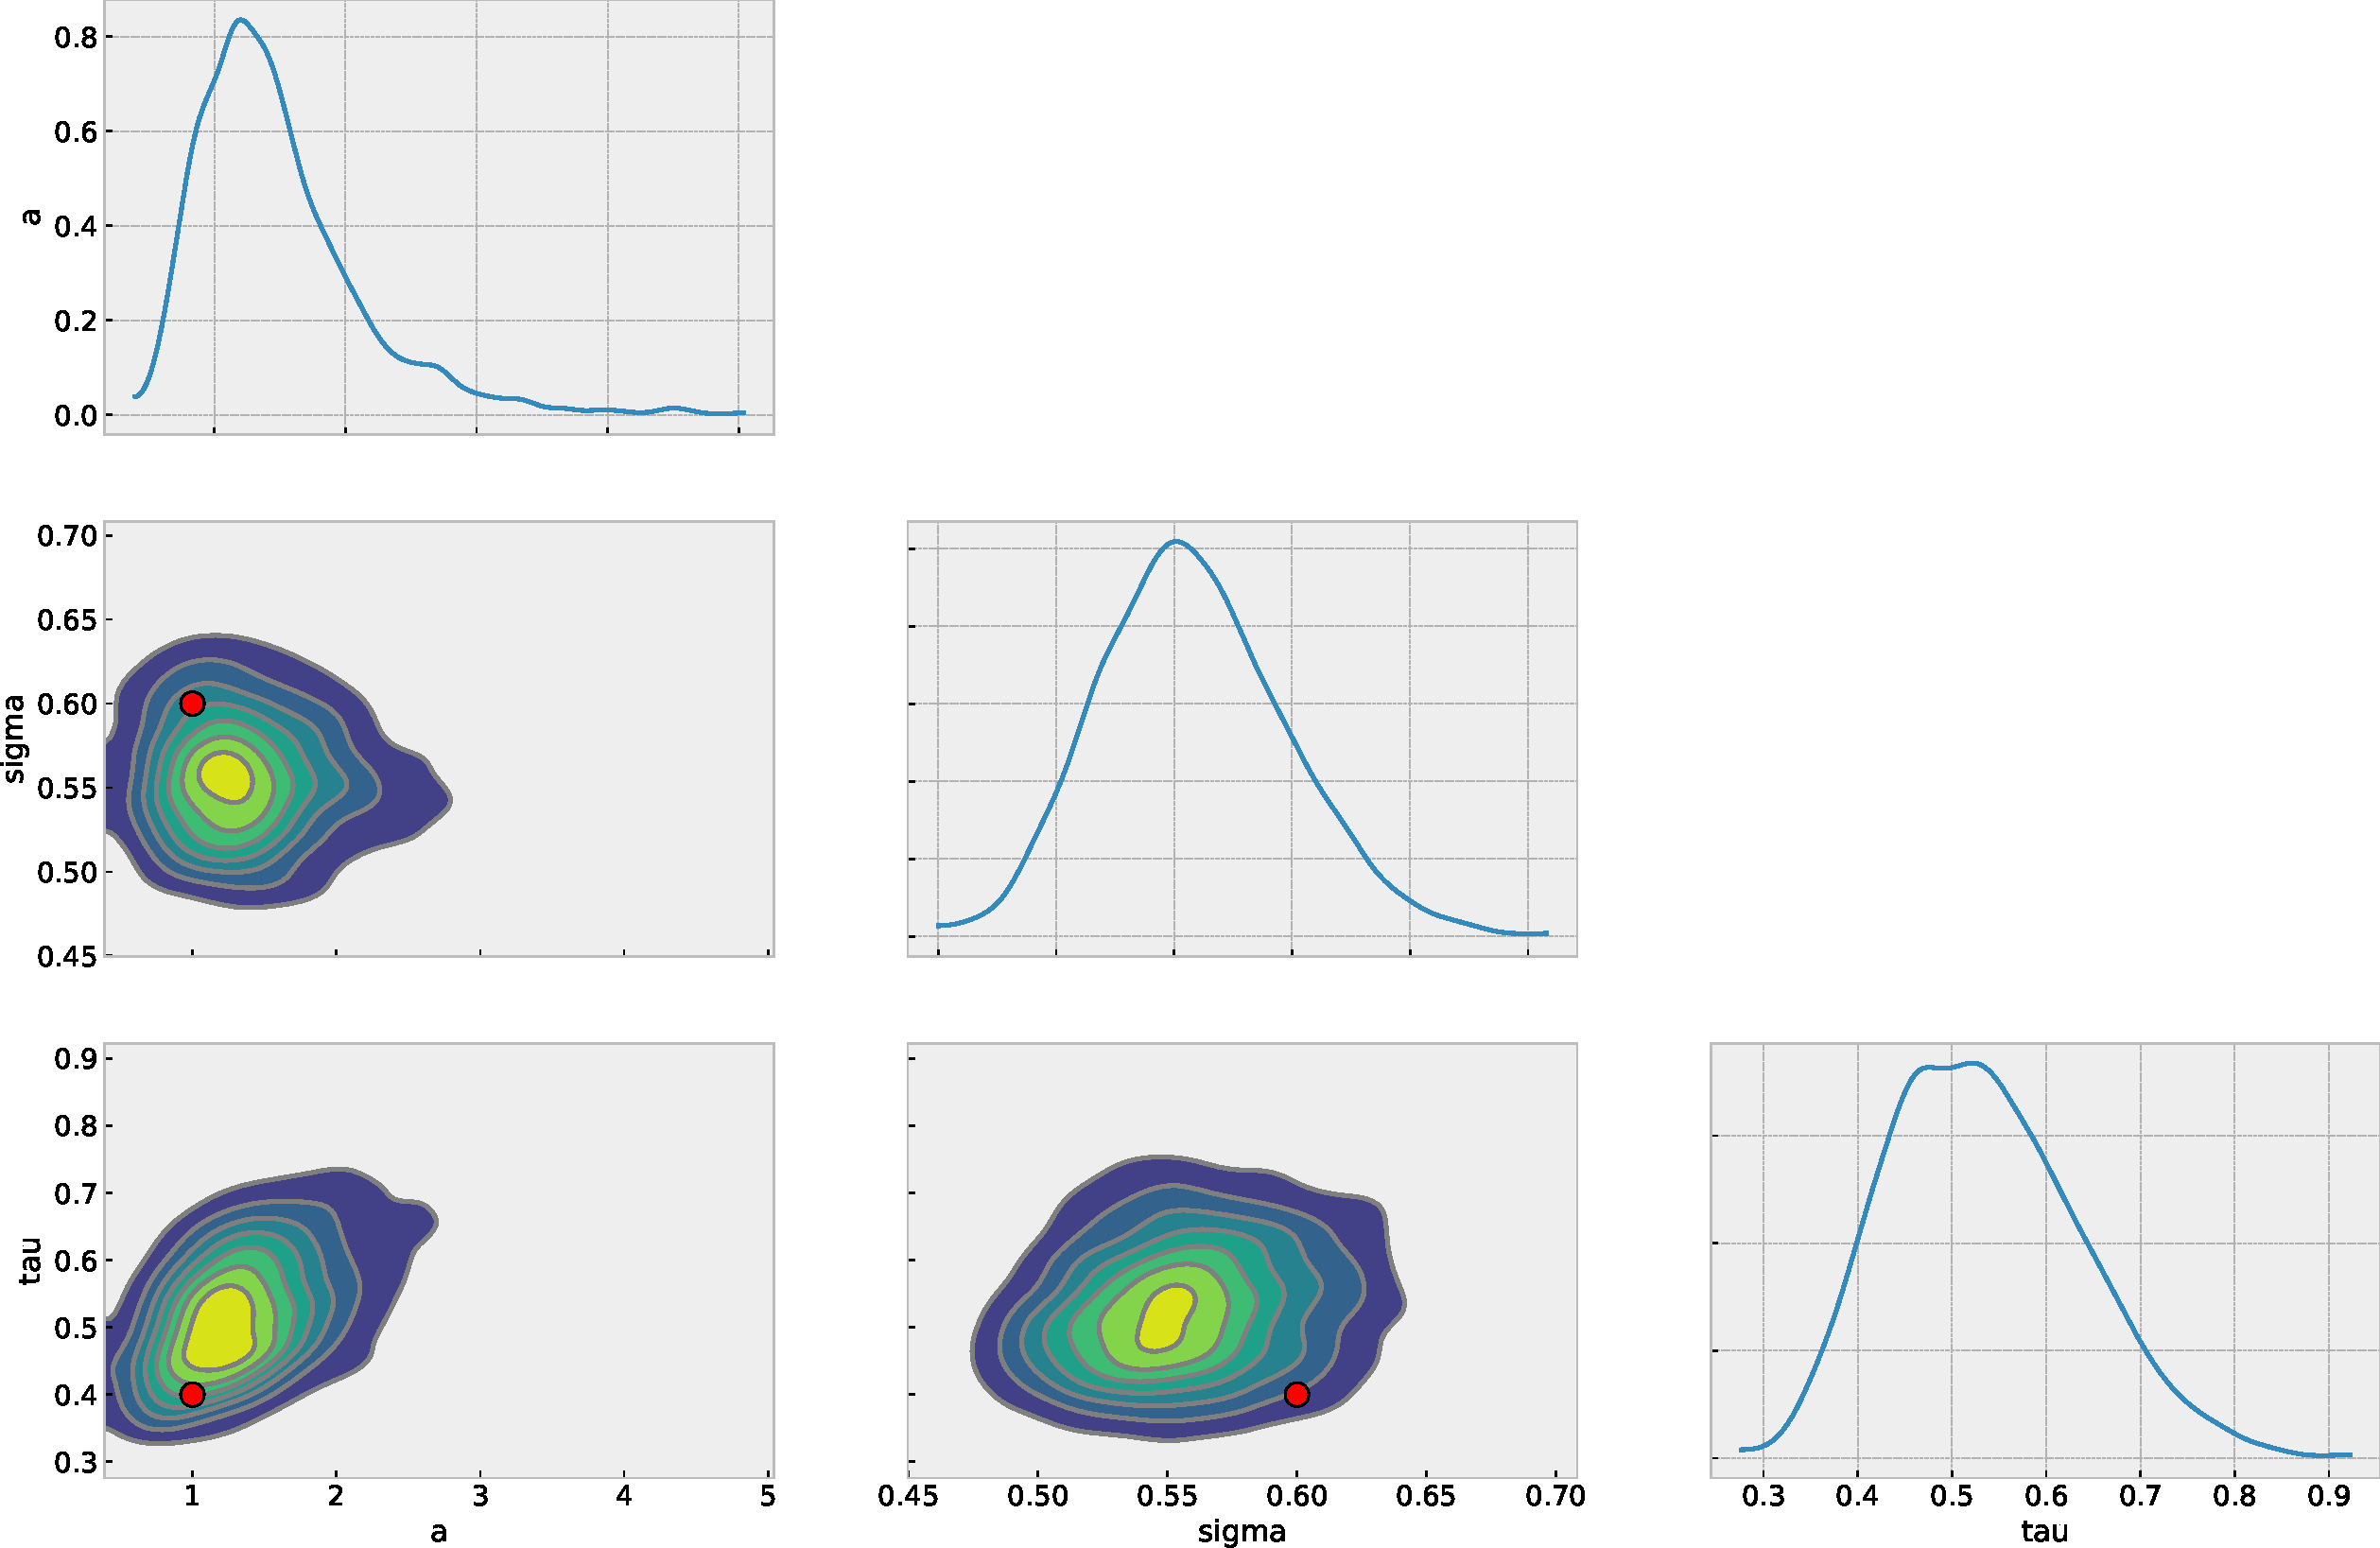
\includegraphics[width=\linewidth]{fig/gp/gp2.pdf}
\caption{\label{fig:gp2}}
\end{center}
\end{figure}
ところで、式(\ref{eq:gpmodel0})という観点のモデル化では、$\xv=\zerov$がモデル平均である。credible intervalを計算したものが図\ref{fig:gp3}となっているが、このことが直感的にわかる。
\begin{figure}[htb]
\begin{center}
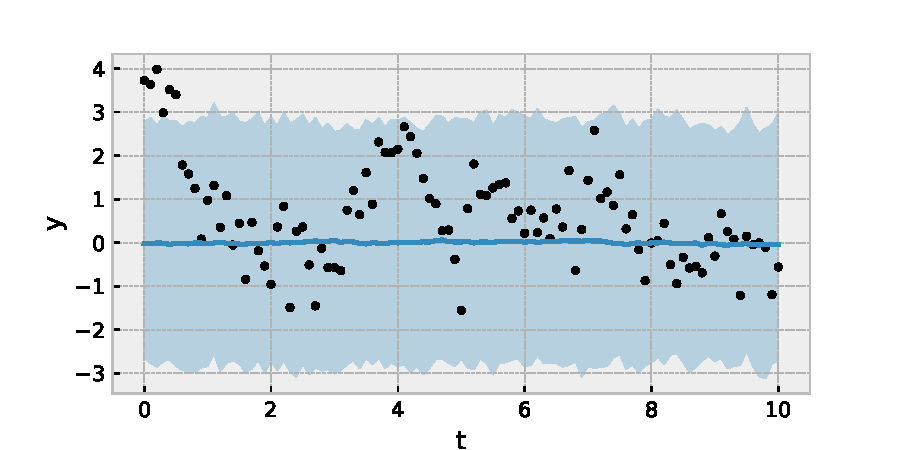
\includegraphics[width=\linewidth]{fig/gp/gp3.pdf}
\caption{\label{fig:gp3}}
\end{center}
\end{figure}


\subsection*{モデルとしてのガウス過程}

上記のガウス過程による解析は、モデルパラメタ$\mv$の事前分布(プライア)として
\begin{align}
p(\mv) = \Ng (\zerov,\Sigma)
\end{align}
と置き、
\begin{align}
d_i &= m_i + \epsilon \\
\epsilon &\sim \Ng (0,\sigma^2)
\end{align}
と見ることもできる。ここに$\epsilon$は観測ノイズに対応している。もう少しまどろっこしく書くとモデル$\gv$を恒等変換として、
\begin{align}
\label{eq:identif}
\gv(\mv) &= \mv \\
\dv &= \gv(\mv) + \epsilonv \\
\epsilonv &\sim \Ng (\boldsymbol{0} ,\sigma^2 I)
\end{align}
のように書ける。この場合、尤度関数が
\begin{align}
p(\dv|\mv) &= \Ng (\dv;\gv(\mv),\sigma^2 I) = \Ng (\dv;\mv,\sigma^2 I)
\end{align}
となる。そして、さらにこの事前分布の中にパラメタがあるという構造となっている。つまり
\begin{align}
\Sigma_{ij} = a k(|t_i-t_j|;\tau) 
\end{align}
としていて、このパラメタ$a$,$\tau$をハイパーパラメタという。そしてハイパーパラメタの事前分布(超事前分布またはハイパープライア)をさらに仮定するということに相当する。



ハイパーパラメタを固定した状態では、$\mv$の事後分布を解析的に書けることが知られている。ここでガウス過程の計算法を紹介しよう。まず多変数正規分布に多変数正規分布をかけても多変数正規分布である。そこで計算しなくてはならないのはexpのべきの部分のみである。多変数正規分布の「べき」部分は
\begin{align}
\label{eq:gp}
&- 2 \log{ \Ng(\mv;\muv, \Sigma) } = (\mv - \muv)^\top \Sigma^{-1} (\mv - \muv) \nonumber \\
&= \mv^\top \Sigma^{-1} \mv - 2 \mv^T \Sigma^{-1} \muv + \mathrm{const}. 
\end{align}
となっていることに注意すると、もしある多変数正規分布に従うことがわかっている確率密度分布$p(\mv)$が
\begin{align}
\label{eq:gpqu}
- 2 \log{ p(\mv) } = \mv^\top P \mv - 2 \mv^\top \qv + \mathrm{const},
\end{align}
のように書けたとすると、式(\ref{eq:gp})と比べることで、この確率密度分布は
\begin{align}
\label{eq:gpqusol}
p(\mv) = \Ng(\mv; P^{-1} \qv ,P^{-1}).
\end{align}
であることがわかる。

さて、いま事後分布は
\begin{align}
\label{eq:gppos}
p(\mv|\dv) \propto p(\dv|\mv) p(\mv) = \Ng (\dv;\mv,\sigma^2 I) \Ng (\mv;\zerov,\Sigma)
\end{align}
であるので、この「べき」部分を$\mv$について展開することで、
\begin{align}
\label{eq:gpposs}
&- 2 \log{[\Ng (\dv;\mv,\sigma^2 I) \Ng (\mv;\zerov,\Sigma)]} \nonumber \\
&= \mv^\top (\Sigma^{-1} + \sigma^{-2} I ) \mv - 2 \sigma^{-2} \mv^\top \dv + \mathrm{const.} 
\end{align}
と書けること、また
\begin{align}
\label{eq:gppossxx}
(\Sigma^{-1} + \sigma^{-2} I )^{-1} = \Sigma (I + \sigma^{-2} \Sigma )^{-1}
\end{align}
より
\begin{align}
\label{eq:gpposss}
p(\mv|\dv) = \Ng (\mv;\Sigma (\sigma^{2} I + \Sigma )^{-1} \dv, \Sigma (I + \sigma^{-2} \Sigma )^{-1} )
\end{align}
であることがわかった。

MCMCにより$\tau$と$\sigma$のサンプリングをすることができるが、これらのパラメタの事後分布は何を意味するか考えよう。これらは今の枠組みではハイパーパラメタとみなせるので、まとめて$\thetav = (a, \tau, \sigma)^\top$をハイパーパラメタとおく。ここからは$\thetav$も確率に入れて考えることにする。さて、今、$\mv$について周辺化した尤度
\begin{align}
\label{eq:gppozz}
p(\dv|\thetav) = \frac{p(\dv|\mv,\thetav) p(\mv,\thetav)}{p(\mv|\dv,\thetav)}
\end{align}
はやはり多変数正規分布となるが、また「べき」部分の$\dv$に関する部分だけ考えることにより
\begin{align}
\label{eq:gppozzp}
&- 2 \log p(\dv|\thetav) = \nonumber \\
&- 2 \log p(\dv|\mv,\thetav) + 2 \log p(\mv|\dv,\thetav) + \mathrm{const} \nonumber \\
&= - 2 \log \Ng(\dv|\mv, \sigma^2 I )  \nonumber \\
&+ 2 \log \Ng(\mv|\Sigma (\sigma^{2} I + \Sigma )^{-1} \dv, \Sigma (I + \sigma^{-2} \Sigma )^{-1} ) \nonumber \\
&= \dv^\top (\sigma^{2} I + \Sigma)^{-1} \dv + \mathrm{const.}
\end{align}
である。よって
\begin{align}
\label{eq:gmarg}
p(\dv|\thetav) =  \Ng (\dv; \zerov, \Sigma + \sigma^{2} I )
\end{align}
となる。
\underline{$\Sigma = K(\tau)$とすれば、式(\ref{eq:gpmodel0})と同じである。} 
すなわち、(超)事前分布として$p(\thetav)$を与えた時の周辺化事後分布
\begin{align}
\label{eq:gmpost}
p(\thetav|\dv) \propto p(\dv|\thetav) p(\thetav)
\end{align}
をサンプリングしていることになる。

図\ref{fig:gp2}はハイパーパラメタ$\tau$、$\sigma$の周辺化事後分布を示していることがわかった。つまり$k=0,..., N_s-1$に対して
\begin{align}
\label{eq:gmposts}
\thetav^\dagger_k \sim p(\thetav|\dv) \propto p(\dv|\thetav) p(\thetav)
\end{align}
をサンプリングしたことになる。さて、ではこのサンプルと式(\ref{eq:gpposss})を用いて、
\begin{align}
\label{eq:gpposssaq}
p(\mv, \thetav|\dv) = p(\mv|\thetav, \dv) p(\thetav|\dv)
\end{align}
であることから
\begin{align}
\label{eq:gpposssaahuq}
 p(\mv|\thetav^\dagger_k, \dv) &= \Ng ( \muv_k ,  K_k ) \\
 \label{eq:muvk}
 \muv_k &= K(a^\dagger_k,\tau^\dagger_k) ((\sigma^\dagger_k)^{2} I + K(a^\dagger_k,\tau^\dagger_k) )^{-1} \dv \\
  \label{eq:Kk}
 K_k &= K(a^\dagger_k,\tau^\dagger_k)(I + (\sigma^\dagger_k)^{-2} K(a^\dagger_k,\tau^\dagger_k) )^{-1} 
\end{align}
からサンプルした$\mv^\dagger_k$と$\thetav^\dagger_k$のセットは
\begin{align}
\label{eq:gpposssaqp}
(\mv^\dagger_k,\thetav^\dagger_k) \sim p(\mv, \thetav|\dv) 
\end{align}
とみなせることがわかる\footnote{ハイパーパラメタの点推定(いわゆるmaximum marginal likelihood=maximum evidence)を用いる方法については解説が多くあるが、周辺化事後分布から再サンプリングする議論についてはいまのところ文献が見つからない。ベイズ線形問題+ガウス過程の枠組みで以前、筆者が議論したことがあるので参考までに挙げておく\cite{2020ApJ...900...48K}。}。

HPDIを計算することで、図\ref{fig:gp4}の$\mv$のcredible intervalが求まる。ここで注意点としては、これはモデル$\mv$の90\% intervalであり、観測ノイズ部分を含んだ$\dv$の予測ではないという点である。
\begin{figure}[htb]
\begin{center}
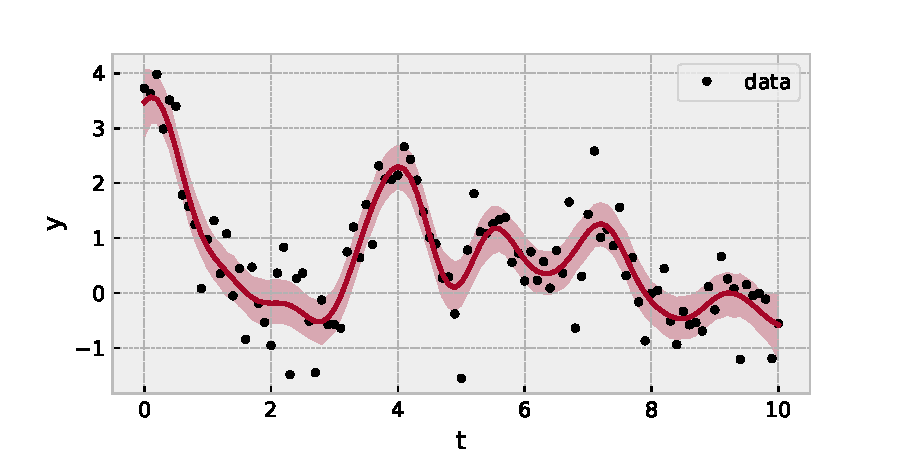
\includegraphics[width=\linewidth]{fig/gp/gp4.pdf}
\caption{\label{fig:gp4}}
\end{center}
\end{figure}

\subsection*{データ点にない位置の予測}

さて、一般に$t=t^\ast$での予測値はどうなるだろうか?以下では再度ハイパーパラメタを省略して表記する。まず、$\mv$、$\mva$がガウス過程に従うとき
\begin{align}
p(\mva|\mv) = \Ng (K_{\times}^\top K^{-1}  \mv, K_\ast - K_\times^\top K^{-1} K_\times)
\end{align}
である。ここに
\begin{align}
K_{ij} &= a k(|t_i-t_j|;\tau) \\
(K_{\times})_{ij} &= a k(|t_i-t^\ast_j|;\tau) \\
(K_{\ast})_{ij} &= a k(|t^\ast_i-t^\ast_j|;\tau) 
\end{align}

同様に
\begin{align}
\label{eq:predgp1}
p(\mva|\dv) =  \Ng (K_{\times}^\top K_\sigma^{-1}  \dv, K_{\ast} - K_\times^\top K_\sigma^{-1} K_\times)
\end{align}
となる。ここに
\begin{align}
(K_{\sigma})_{ij} = a k(|t_i-t_j|;\tau) + \sigma^2 \delta_{i,j}
\end{align}
($\delta_{i,j}$はクロネッカーデルタ)。ここで$p(\mva|\dv)$はあくまでモデルパラメタとしてのガウス過程の事後分布なので、観測ノイズの分は考慮されていない。

もし観測ノイズを含んだ予測を行いたいのならば、
\begin{align}
\dv^\ast = \mv^\ast + \epsilonv
\end{align}
というモデルに基づき、
\begin{align}
\label{eq:predgp2}
p(\dv^\ast|\dv) =  \Ng (K_{\times}^\top K_\sigma^{-1} \dv, K_{\ast,\sigma} - K_\times^\top K_\sigma^{-1} K_\times)
\end{align}
となるだろう。ここに
\begin{align}
(K_{\ast,\sigma})_{ij} &= a k(|t^\ast_i-t^\ast_j|;\tau) + \sigma^2 \delta_{i,j}
\end{align}
である。

というわけで、ハイパーパラメタ込みのサンプリングで式(\ref{eq:predgp1},\ref{eq:predgp2})のサンプリングを行いCredible Intervalを求める。同様にHPDIを求めたものが図\ref{fig:gp6}である。濃い色が$\mva$の、薄い色が$\dv^\ast$のcredible intervalである。

\begin{figure}[htb]
\begin{center}
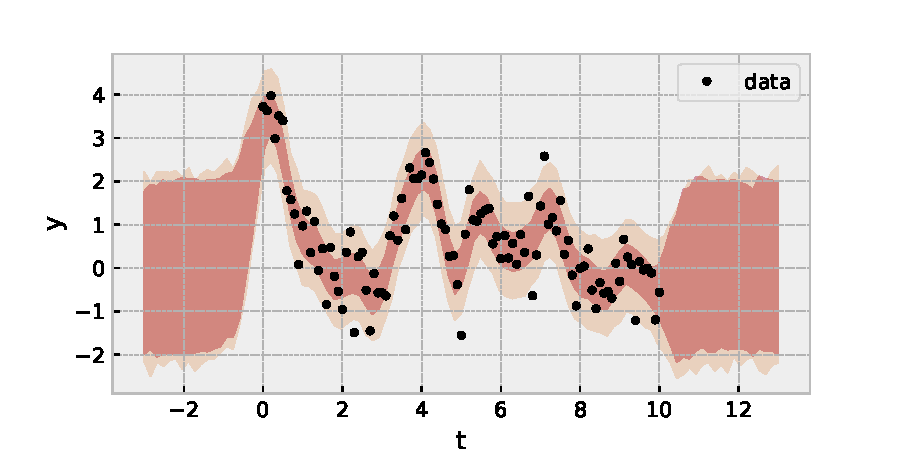
\includegraphics[width=\linewidth]{fig/gp/gp6.pdf}
\caption{\label{fig:gp6}}
\end{center}
\end{figure}

\section{ガウス過程ノイズを含んだモデルフィット$^\ddagger$}

さて、ここまではモデルとしては平均値がゼロのガウス過程により生成されるモデル
\begin{align}
\mv \sim \Ng ({\bf 0},\Sigma(\tv)) 
\end{align}
を考えていた。ここでは一般に平均値が$t$の関数となるガウス過程によりデータが生成される場合を考えよう。すなわち
\begin{align}
\label{eq:modelgp}
\mv \sim \Ng (\fv(\tv),\Sigma(\tv)) 
\end{align}
の場合を考えよう。ここに$\fv(\tv)$は$f(t)$に対し、$\tv=(t_0,t_1,\cdots t_{N-1})$を要素ごとに適用したベクトル版である。ここでは$f(t)$として
\begin{align}
f(t) = k e^{-(t-T_0)^2/2 s^2} \sin{(2 \pi t/P)}
\end{align}
というものを考えてみよう。上では簡単に$f(t)$と書いたが、パラメタを$\thetav=(T_0,k,s,P)$として$f(t;\thetav)$という表記も併用する。

式(\ref{eq:modelgp})の共分散行列をRBFカーネルとして選択すると、例えば、図\ref{fig:gp1m}上のようなデータが生成される。ここで$\tau=3$であり$f(t)$より比較的ゆったりとしたトレンドが乗っているのが見て取れるだろう。
\begin{figure}[htb]
\begin{center}
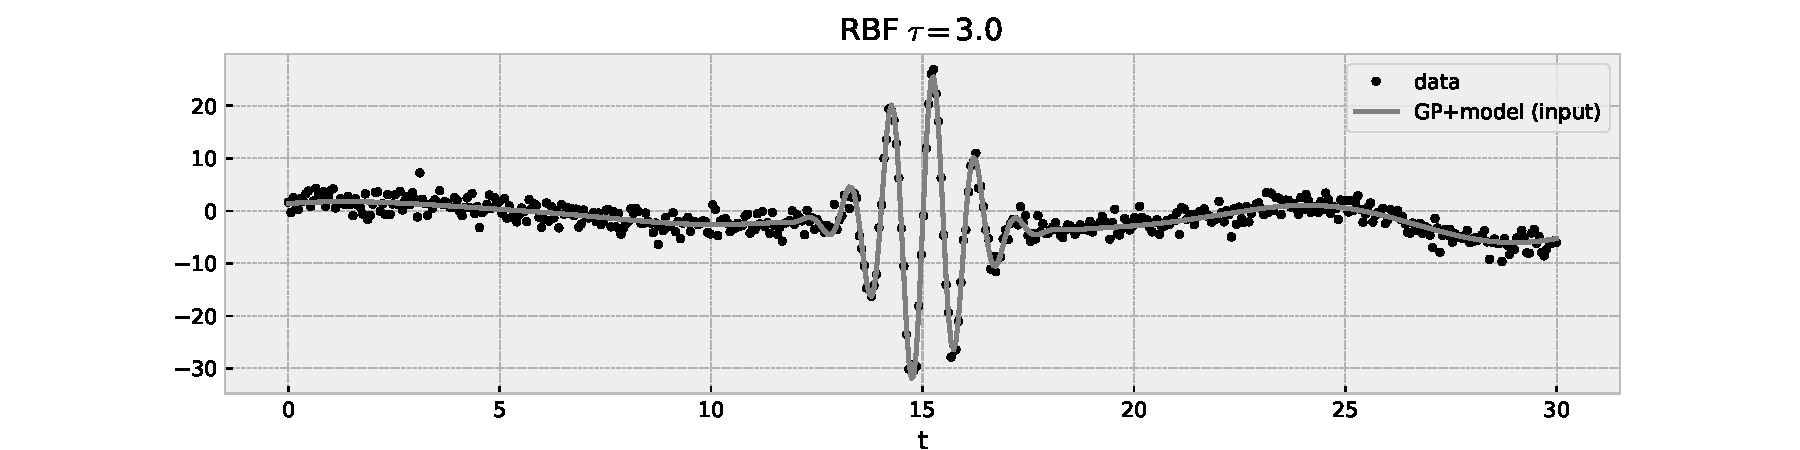
\includegraphics[width=\linewidth]{fig/gpmodel/gp1.pdf}
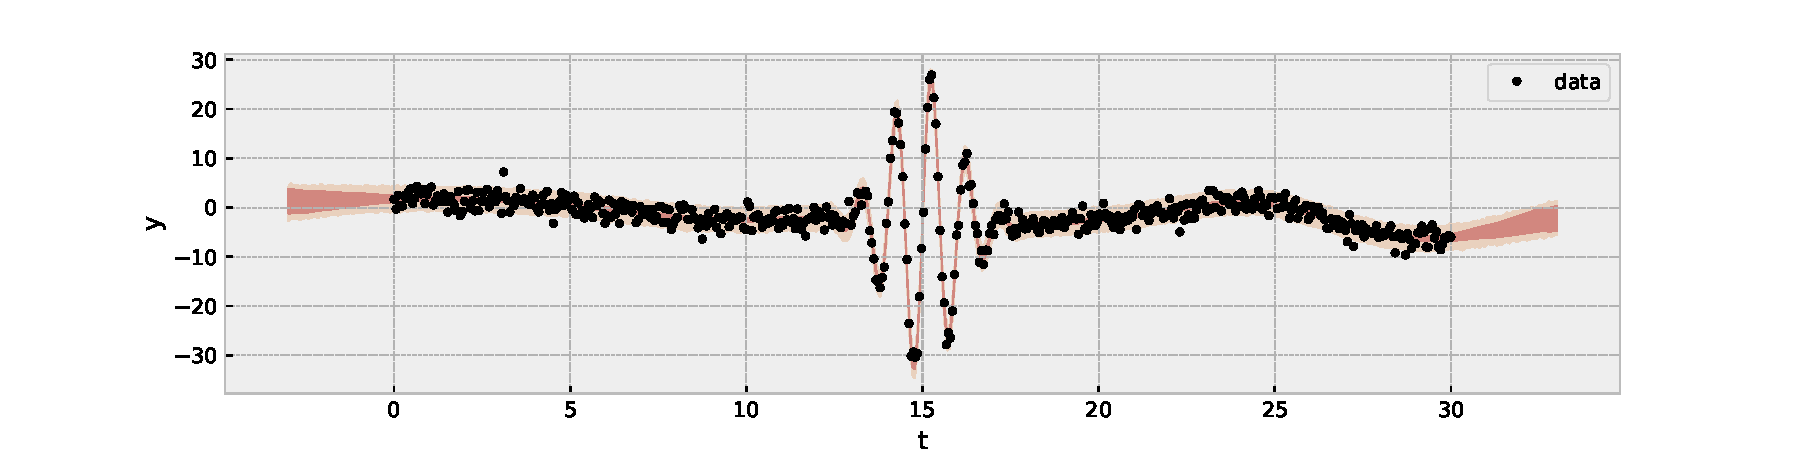
\includegraphics[width=\linewidth]{fig/gpmodel/gp6.pdf}
\caption{実線は$\sigma$の観測ノイズなし。\label{fig:gp1m}}
\end{center}
\end{figure}
このようなモデルをHMCフィットするというのは、シグナル$f(t)$と相関のあるノイズ+観測ノイズをモデル化し、$f(t)$の持つパラメタを推定したいときに対応する。


$\fv(\tv)$がわかっている場合、観測ノイズを含まない、および、含んだ予測は、それぞれ、
\begin{align}
\label{eq:predgp_model}
&p(\mva|\dv) =   \nonumber \\
&\Ng (\fv(\tv^\ast) + K_{\times}^\top K_\sigma^{-1}  (\dv - \fv(\tv)),  K_{\ast} - K_\times^\top K_\sigma^{-1} K_\times) \\
&p(\dv^\ast|\dv) =   \nonumber \\
&\Ng (\fv(\tv^\ast) + K_{\times}^\top K_\sigma^{-1} (\dv - \fv(\tv)), K_{\ast,\sigma} - K_\times^\top K_\sigma^{-1} K_\times)
\end{align}
となる。$\fv(t)$の持つパラメタ$\thetav=(T_0,k,s,P)$はHMCでサンプリングされるから、例えば後者なら、サンプリングされた各$\thetav^\dagger_k$をもちいて
\begin{align}
\label{eq:predgp2_}
&\dv^\ast_k \sim  \Ng (\mu_k, K_k) \\
&\mu_k = \fv(\tv^\ast; \thetav^\dagger_k) + K_{\times}^\top K_\sigma^{-1} (\dv - \fv(\tv; \thetav^\dagger_k)) \\
&K_k = K_{\ast,\sigma} - K_\times^\top K_\sigma^{-1} K_\times
\end{align}
をサンプリングすれば、予測のサンプリングができる。というわけで、以下のようにモデル$f(t)$込みのGPのフィットを行うことができる(図\ref{fig:gp1m}下)。

